\subsection{Použitie hybridných modelov}
V predchádzajúcich častiach sme ukázali ako si s problematikou optimalizácie prevádzky zariadenia, pri nepresnom matematickom opise, dokázali poradiť dvojkroková optimalizácia a schéma úpravy modifikátora. Poďme sa pozrieť ako sa s touto problematikou dokáže vysporiadať prístup s použitím hybridných modelov.

V teoretickej časti sme spomenuli, že aj v rámci hybridného modelovania môžeme k tejto problematike pristupovať rôzne a to na základe meraných údajov. V skutočnosti by sme nedokázali získať relevantné dáta koncentrácie biomasy, nie v taktom množstve a kvalite, aby sme pomocou nich mohli identifikovať dátový model. Preto sa budeme venovať najmä výsledkom hybridných modelov, ktoré sme získali na základe údajov o koncentrácii substrátu. Ďalším dôvodom, prečo sme sa takto rozhodli je aj fakt, že výsledok oboch prístupov je viacmenej rovnaký a to môžeme sledovať na Obr. \ref{fig:hybrid_costFuns_compar}. Na obrázku je znázornený priebeh optím hybridných modelov identifikovaných na dátach biomasy aj substrátu počas desiatich iterácií. Jednotlivé optimá sme vyjadrili ako hodnoty účelovej funkcie zariadenia. Bodkovaná čiara znázorňuje skutočný optimálny stav zariadenia. Ako si môžno všimnúť, tak v oboch prípadoch nenastal takmer žiaden posun od optimálneho stavu mechanického modelu. 
\begin{figure}
	\centering
	\begin{subfigure}[b]{0.49\textwidth}
		\centering
		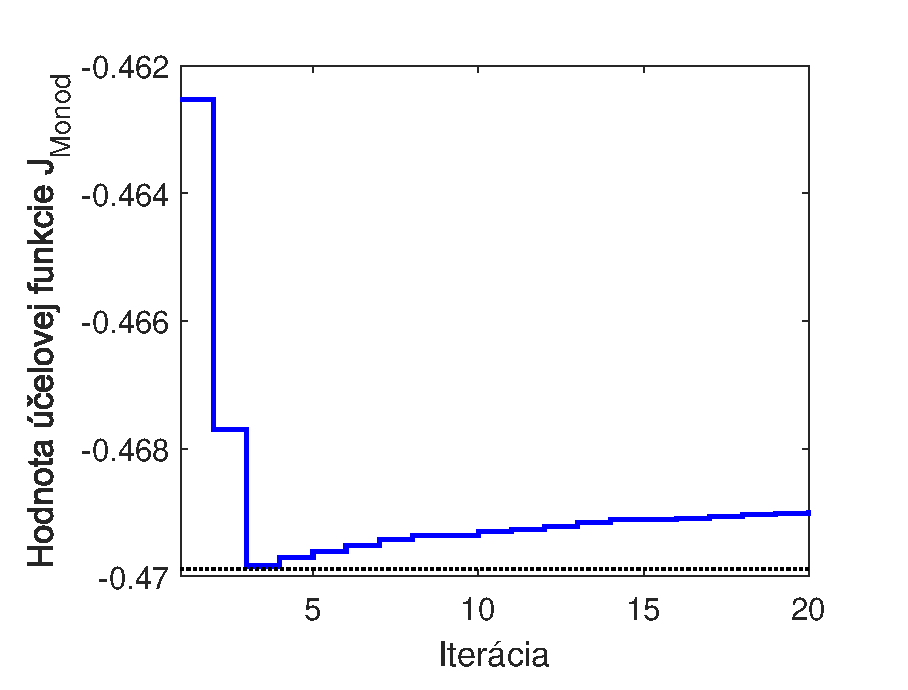
\includegraphics[width=\linewidth]{images/hybrid_bio_costFun}
		\caption{}
		\label{fig:hybrid_bio_costFun}
	\end{subfigure}
	\hfill
	\begin{subfigure}[b]{0.49\textwidth}
		\centering
		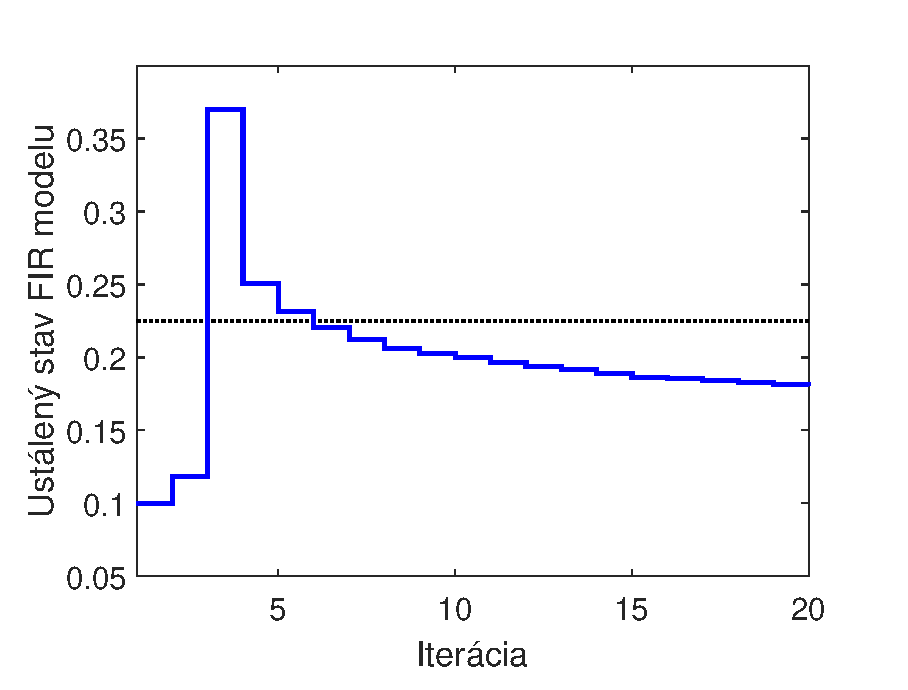
\includegraphics[width=\linewidth]{images/hybrid_bio_ss}
		\caption{}
		\label{fig:hybrid_bio_ss}
	\end{subfigure}
	\bigskip
	\begin{subfigure}[b]{0.49\textwidth}
		\centering
		\includegraphics[width=\linewidth]{images/hybrid_bio_order}
		\caption{}
		\label{fig:hybrid_bio_order}
	\end{subfigure}
	\caption{text}
	\label{fig:hybrid_bio_opt_results}	
\end{figure}

Je zrejmé, že nová rýchlosť riedenia $ D $ získaná na základe hybridného modelu v prvej--druhej iterácii, nepriniesla skokovú zmenu, ktorá by bola výraznejšia ako vplyv šumu merania, tým pádom bude náš dátový model predikovať konštantnú hodnotu ustáleného stavu. Toto môžeme sledovať na Obr. \ref{fig:hybrid_FIRsub_ss}, kde je zobrazený priebeh rozdielu odhadnutého ustáleného stavu koncentrácie substrátu medzi zariadením a nominálnym modelom. Bodkovanou čiarou je znázornená hodnota rozdielu oboch modelov v optimálnom režime zariadenia. Tým že sa nemení informačná výdatnosť údajov, nemení sa ani rád modelu a to je ukázané na vedľajšom obrázku \ref{fig:hybrid_FIRsub_order}. Pripomenieme, aby FIR model v sebe uchoval informácie o nelinearite systému, musí zväčšovať svoj rád. 
\begin{figure}
	\centering
	\begin{subfigure}[b]{0.49\textwidth}
		\centering
		\includegraphics[width=\linewidth]{images/hybrid_sub_costFun}
		\caption{}
		\label{fig:hybrid_sub_costFun}
	\end{subfigure}
	\hfill
	\begin{subfigure}[b]{0.49\textwidth}
		\centering
		\includegraphics[width=\linewidth]{images/hybrid_sub_ss}
		\caption{}
		\label{fig:hybrid_sub_ss}
	\end{subfigure}
	\bigskip
	\begin{subfigure}[b]{0.49\textwidth}
		\centering
		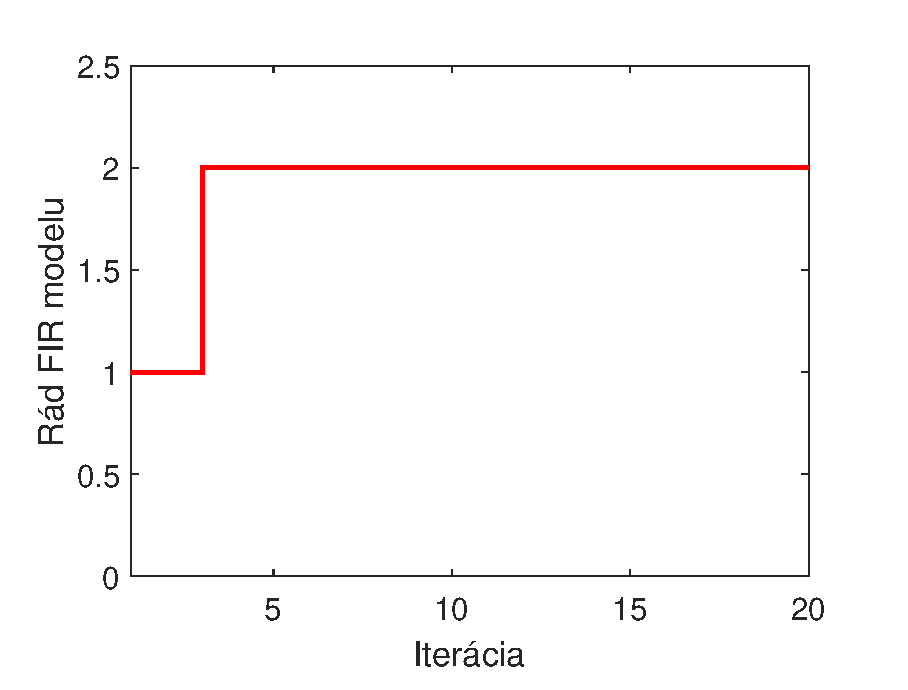
\includegraphics[width=\linewidth]{images/hybrid_sub_order}
		\caption{}
		\label{fig:hybrid_sub_order}
	\end{subfigure}
	\caption{text}
	\label{fig:hybrid_sub_opt_results}	
\end{figure}

\begin{figure}
	\centering
	\includegraphics[width=0.7\linewidth]{images/hybrid_sub_and_bio_compar}
	\caption{}
	\label{fig:hybrid_sub_and_bio_compar}
\end{figure}

Zistili sme, že takýmto štýlom sa nedokážeme posunúť k optimálnemu stavu zariadenia. Dátové časti hybridných modelov majú veľkú výhodu a tou je, že ich môžeme natrénovať na historických údajoch dopredu. Takto už bude mať dátový model nejaké informácie o systéme v sebe uchované dopredu, zlepšia sa predikčné vlastnosti modelu, a tým by sa mohla obohatiť aj informačná výdatnosť generovaných údajov.

Výsledok tohto prístupu môžeme vidieť na Obr. \ref{fig:hybrid_FIR_multipleStep_costFun}, kde FIR model sme identifikovali pomocou dát, ktoré sú zobrazené na Obr. \ref{fig:hybrid_FIR_multipleStep_data}. Môžeme si všimnúť, že v prvej iterácii sme dosiahli výrazný skok ku optimu zariadenia. V ďalších iteráciách sme však skonvergovali späť k pôvodnému riešeniu. Problémom je, že použitý FIR model si pamätá hodnotu ustáleného stavu pri poslednej skokovej zmene, ktorá sa automaticky stane aj jeho novým ustáleným stavom. Keďže naše dáta boli vygenerované na základe skokovej zmeny vo vstupnej veličine $ D = \lbrace 0.3760, 0.3845, 0.3930, 0.4015, 0.4100 \rbrace \si{\per\hour} $, ktorá bola zoradená vzostupne, tak posledný ustálený stav zodpovedá práve najväčšiemu rozdielu koncentrácií substrátu. Táto hodnota nás potom posunula bližšie k optimu zariadenia ($ D = 0.3833\si{\per\hour} $), ale táto hodnota rýchlosti riedenia bola nižšia ako posledná z dát na trénovanie modelu, čo viedlo k nižšej hodnote ustáleného stavu a preto sme sa opäť začali vzďaľovať od optimálneho chodu zariadenia.
\begin{figure}
	\centering
	\begin{subfigure}[b]{0.49\textwidth}
		\centering
		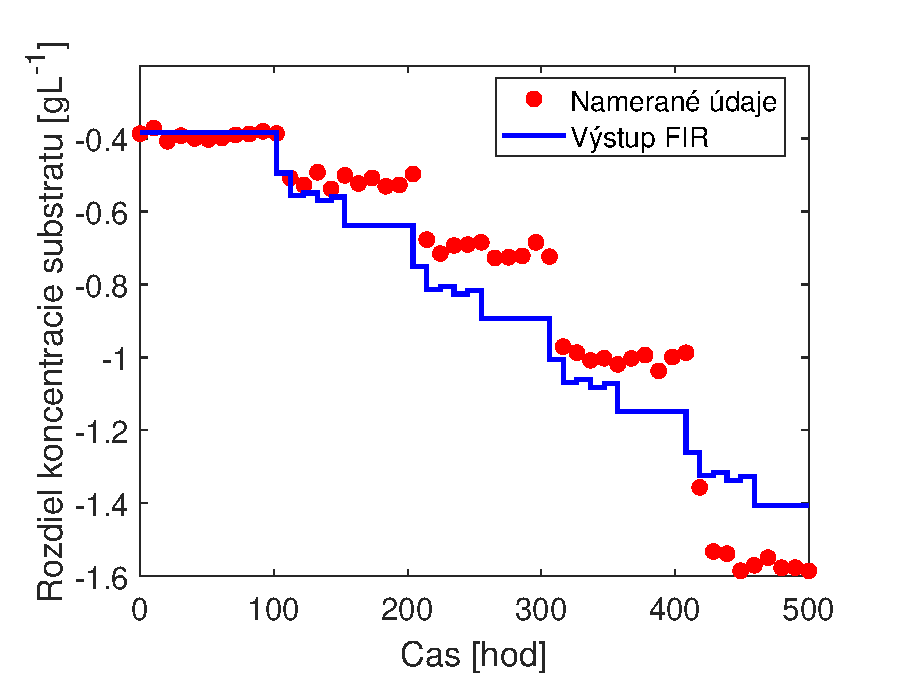
\includegraphics[width=\linewidth]{images/hybrid_multipleStep_data}
		\caption{Trénovacie dáta a výstup FIR modelu.\newline \newline}
		\label{fig:hybrid_multipleStep_data}
	\end{subfigure}
	\hfill
	\begin{subfigure}[b]{0.49\textwidth}
		\centering
		\includegraphics[width=\linewidth]{images/hybrid_multipleStep_costFun}
		\caption{Optimá hybridného modelu vyjadrené ako hodnoty účelovej funkcie Monod modelu (zariadenia).}
		\label{fig:hybrid_multipleStep_costFun}
	\end{subfigure}
	\caption{Priebeh optimalizácie zariadenia pomocou hybridného modelovania, ktorého dátová časť bola vopred natrénovaná na dátach z viacnásobnej skokovej zmeny $ D = \lbrace 0.3760, 0.3845, 0.3930, 0.4015, 0.4100 \rbrace \si{\per\hour} $.}
	\label{fig:hybrid_multipleStep_approach}
\end{figure}

Predstavme si teraz situáciu, že poznáme optimálnu rýchlosť riedenia zariadenia $ D_{P}^{\star} $. Ak spravíme skokovú zmenu z hociktorého ustáleného stavu na optimálnu hodnotu zariadenia, mali by sme získať presný rozdiel v koncentrácii substrátu, ktorý by nás z daného ustáleného stavu mal dostať do optimálneho stavu zariadenia. Pokúsme sa na týchto dátach natrénovať dátovú časť hybridného modelu a pozrime sa ako dopadne optimalizácia prevádzky zariadenia. 

Vykonali sme skokovú zmenu z ustáleného stavu nominálneho modelu pri rýchlosti riedenia $ D_{N}^{\star} = 0.3760\si{\per\hour} $ na hodnotu zodpovedajúcu optimálnej prevádzke zariadenia $ D_{P}^{\star} = 0.3974\si{\per\hour} $. Rozdiel v koncentrácii ustálených stavov substrátu pri tejto rýchlosti riedenia bol $ \Delta_{s} = -0.8448\si{\gram\per\liter} $ a FIR model identifikovaný pomocou týchto dát predikoval hodnotu rozdielu ustáleného stavu $ \Delta_{s}^{FIR} = -0.8360\si{\gram\per\liter} $. Ak máme k dispozícii presný rozdiel ustáleného stavu koncentrácie substrátu pri optimálnej rýchlosti riedenia zariadenia $ D_{P}^{\star} $, tak účelová funkcia hybridného modelu a zariadenia musia mať spoločný prienik v optime a to môžeme vidieť na Obr. \ref{fig:hybrid_and_monod_opt_compar}. Avšak, optimum hybridného modelu nedosiahlo hodnotu optimálnej prevádzky zariadenia ako môžeme vidieť na Obr. \ref{fig:hybrid_optimum_shift}. Dôvodom je, že korekcia ustáleného stavu nepresného mechanického modelu pomocou dátového modelu, štýlom aký uvádza rovnica \eqref{eq:hybrid_opt_subs} resp. \eqref{eq:hybrid_opt_bio}, neupravuje účelovú funkciu dostatočným spôsobom, ako môžeme vidieť na Obr. \ref{fig:hybrid_and_monod_opt_compar}. 
\begin{figure}
	\centering
	\begin{subfigure}[b]{0.49\textwidth}
		\centering
		\includegraphics[width=\linewidth]{images/hybrid_optShift_data}
		\caption{}
		\label{fig:hybrid_optShift_data}
	\end{subfigure}
	\hfill
	\begin{subfigure}[b]{0.49\textwidth}
		\centering
		\includegraphics[width=\linewidth]{images/hybrid_optShift_costFunValues}
		\caption{Optimá vyjadrené ako hodnota účelovej funkcie Monod modelu (zariadenia).}
		\label{fig:hybrid_optShift_costFunValues}
		\end{subfigure}
	\caption{Porovnanie optím a účelových funkcií Monod (zaradenia) a hybridného modelu, ktorý bol identifikovaný na dátach zo skokovej zmeny $ D_{N}^{\star} \rightarrow D_{P}^{\star} $.}
	\label{fig:hybrid_optimum_shift}
\end{figure}

\begin{figure}
	\centering
	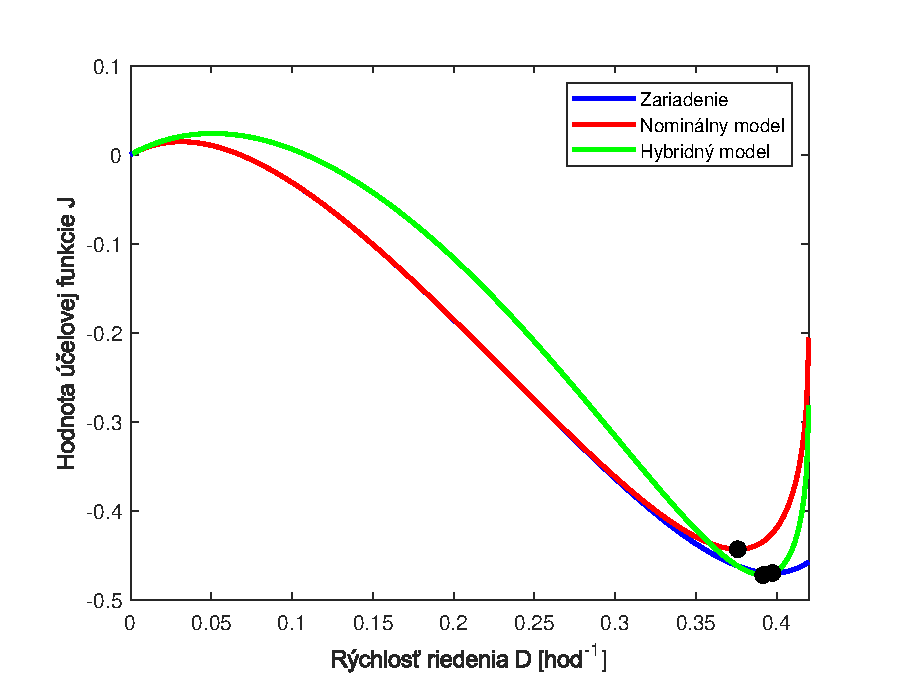
\includegraphics[width=0.7\linewidth]{images/hybrid_and_monod_costFun_compar}
	\caption{}
	\label{fig:hybrid_and_monod_costFun_compar}
\end{figure}

Zväčšením hodnoty rozdielu ustáleného stavu by sme dokázali posunúť optimum hybridného modelu k optimu zariadenia, ale takáto hodnota by nemala nič spoločné s realitou, pretože taký dramatický rozdiel medzi Monod a Haldane modelom nie sme schopný dosiahnuť zmenou rýchlosti riedenia $ D $. Ďalšou možnosťou, akou by sme mohli dosiahnuť optimum prevádzky zariadenia, by mohla byť zmena korekcie nominálneho modelu napr. štýlom, akým to rieši schéma úpravy modifikátora, teda úpravou gradientu účelovej funkcie nominálneho modelu. Takýto prístup by mal viacero výhod a najväčšou by bola skutočnosť, že šum merania by už nebol takým výrazným problémom, akým je pri schéme úpravy modifikátora. Tieto hypotézy by však bolo nutné overiť, čo by mohol byť námet ďalšieho výskumu.